\documentclass[12pt]{book}
\usepackage[margin=.85in]{geometry} % for MARGIN
\usepackage[many]{tcolorbox}    	% for COLORED BOXES (tikz and xcolor included)

\usepackage{multirow}
\usepackage{tabularx}
\usepackage{multicol}   
\usepackage{enumerate}
\usepackage[shortlabels]{enumitem}
\usepackage{varwidth}
\usepackage{tasks}
\usepackage[export]{adjustbox}
\usepackage{array} % For m{} column type

\usepackage{titleps}
\usepackage{setspace}               % for LINE SPACING
\usepackage[⟨options⟩]{fancyhdr}
\usepackage{enumitem}
\setlist{nosep}
\usepackage{tikz}
\usepackage{pgfplots}
\pgfplotsset{compat=1.5.1}
\usetikzlibrary{datavisualization}
\usetikzlibrary{datavisualization.formats.functions}

\newcommand{\D}{\displaystyle}


\setlength\parindent{0pt}   % killing indentation for all the text
\setstretch{1.3}            % setting line spacing to 1.3
\setlength\columnsep{0.25in} % setting length of column separator
\pagestyle{fancy}           % setting pagestyle to be headings

\usepackage[]{titlesec}

\fancyhead[L]{Math V04 - College Algebra}
\fancyhead[R]{Christina Papazacharioudakis}

\tcbset{
    sharp corners,
    colback = white,
    before skip = 0.2cm,    % add extra space before the box
    after skip = 0.5cm      % add extra space after the box
}                           % setting global options for tcolorbox

    \newtcolorbox{boxR}{
    fontupper = \color{black}, % font color
    boxrule = 1.5pt,
    colframe = black,
    rounded corners,
    arc = 5pt   % corners roundness
}



\begin{document}


{\Large \textbf{5.3 Graphs of Polynomial Functions}}
\skip

In the previous section, we made observations on how many possible $x$-intercepts and turning points a polynomial could have. In this section, we will find exactly how many x-intercepts and turning points a polynomial will have.
\vspace{2mm}

{\large \textbf{Using Factoring to Find Zeros of Polynomial Functions}}
\vspace{2mm}

When we had a polynomial function $f(x)$, the $x$-intercepts were found by letting $f(x)=0$. Because we are finding $x$ values that make the function zero, $x$-intercepts are often called ``zeros".

\bigskip

\begin{boxR}
\textbf{How To}
    \vspace{1mm}
    \hline
    \vspace{2mm}
\textbf{Given a polynomial function, $f(x)$, find the $x$-intercepts by factoring.}
\begin{enumerate}
    \item Set $f(x)=0$.
    \item If the polynomial is not given in factored form, factor it.
    \item Set each factor equal to zero and solve to find the $x$-intercepts. 
\end{enumerate}
\end{boxR}
\skip

\underline{\textbf{Example 1 - Find the $x$-Intercepts of a Polynomial Function by Factoring}}

Find the $x$-intercepts of the $f(x)=x^2-3x+2$.

\vspace{10mm}

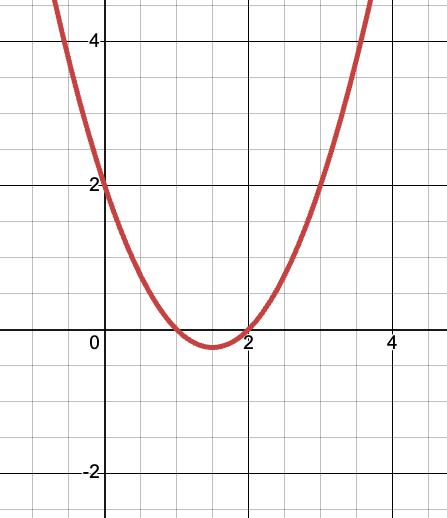
\includegraphics[scale=.4]{Chapter 5/5.3-figure1.png}


\newpage

\underline{\textbf{Example 2 - Find the $x$-Intercepts of a Polynomial Function by Factoring}}

Find the $y$-intercepts and $x$-intercepts of $g(x)=(x-2)^2(2x+3)$.


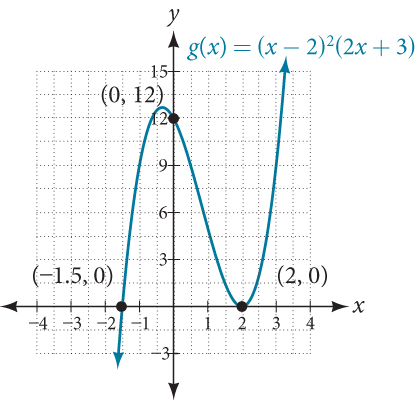
\includegraphics[scale=.5]{Chapter 5/5.3-figure2.jpeg}
\vspace{50mm}

Notice that when a factor had a degree of $1$, then the corresponding zero cross through the $x$-axis, and when a factor had a degree of $2$, then the corresponding zero  ``bounced off" the $x$-axis. Odd powers cut through the $x$-axis and even powers just touch (or ``bounce off") the $x$-axis.
\bigskip

\centerline{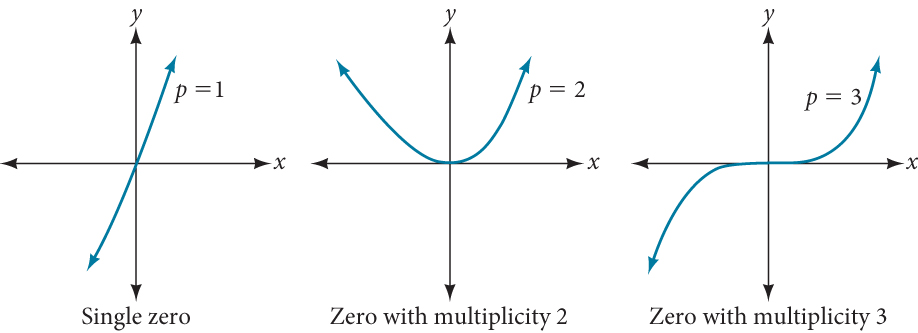
\includegraphics[scale=.4]{Chapter 5/5.3-figure4.jpeg}}



\newpage

Suppose, we graph the function $$f(x)=(x+3)(x-2)^2(x+1)^3$$


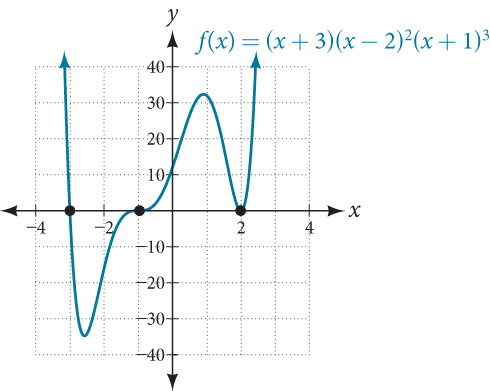
\includegraphics[scale=.45]{Chapter 5/5.3-figure3.jpeg}


\vspace{70mm}
\begin{boxR}
   \textbf{Graphical Behavior of Polynomials at $x$-Intercepts}
    \vspace{1mm}
    \hline
    \vspace{2mm}
    Given a factor of the form $(x+h)^p$, the behavior near the $x$-intercept $-h$ is determined by the power $p$.
  We say that $x=-h$ is a zero of \textbf{multiplicity} $p$.
 \begin{itemize}
     \item If $p$ is even, the graph of the polynomial will touch (or ``bounce off") the $x$-axis at the corresponding zero.
     \item If $p$ is odd, the graph of the polynomial will cross (``cut through") the $x$-axis at the corresponding $x$-value.
 \end{itemize}

The sum of the multiplicities is the degree of the polynomial function.
\end{boxR}

\newpage

\underline{\textbf{Example 3 - Identifying Zeros and their Multiplicities}}

Use the graph of the function of degree $6$ in the figure below to identify the zeros of the function and their multiplicities. 

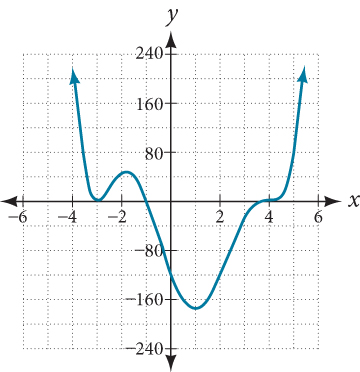
\includegraphics[scale=.5]{Chapter 5/5.3-figure5.jpeg}


\newpage
{\large \textbf{Determining End Behavior}}

As a reminder from last section, we determined the end behavior of a polynomial,
$$ f(x) = a_nx^n + a_{n-1}x^{n-1} + \ldots + a_1x+a_0$$ by focusing on the degree and sign of the leading term, $a_nx^n$. The behavior of the leading term told us the end behavior of the polynomial.

\vspace{5mm}

\centerline{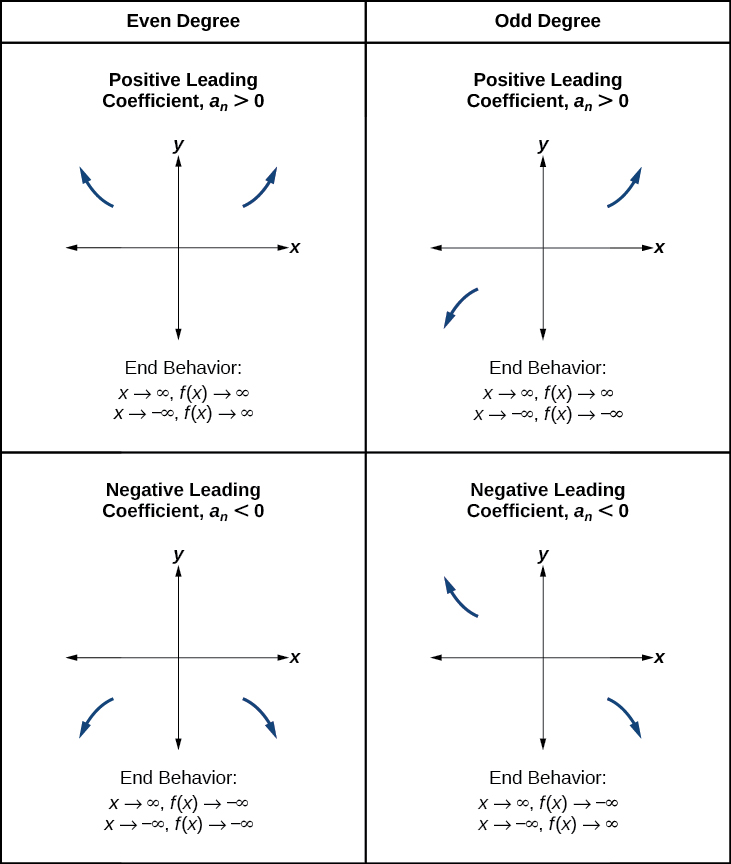
\includegraphics[scale=1]{Chapter 5/5.3-figure6.jpeg}}

The behavior of the polynomial in the middle is determined by its zeros.

Now we put this all together to graph a polynomial...

\newpage

\begin{boxR}
    \textbf{How To}
    \vspace{1mm}
    \hline
    \vspace{2mm}
    \textbf{Given a polynomial function, sketch the graph.}
    \begin{enumerate}
        \item Find the $x$ and $y$ intercepts. 
        \item Determine the behavior of the polynomial at the $x$-intercepts looking at its multiplicity.
        \item Determine the end behavior by examining the leading term.
        \item Combine information about the end behavior and intercepts to sketch the graph.
        \item Ensure that the number of turning points does not exceed one less than the degree of the polynomial.
    \end{enumerate}
\end{boxR}

\vspace{5mm}

\underline{\textbf{Example 4 - Sketching the Graph of a Polynomial Function}}

Sketch the graph of $f(x)=-2(x+3)^2(x-5)$


\newpage

{\large \textbf{Writing Formulas for Polynomial Functions}}

In the previous example, we graphed a polynomial given its function. Now we go the other direction: given the graph of a polynomial, can we find its function?
\bigskip

\begin{boxR}
\textbf{How To}
\vspace{1mm}
\hline
\vspace{2mm}
\textbf{Given a graph of a polynomial function, write a formula for the function.}
\begin{enumerate}
    \item Identify the $x$-intercepts of the graph to find the factors of the polynomial.
    \item Exam the behavior of the graph at the $x$-intercepts to determine the multiplicity of each factor. 
    \item Create the function of a polynomial from the previous step, considering a stretch factor of $a$
    \item Use any other point on the graph ($y$-int may be the easiest) to determine the stretch factor $a$.
\end{enumerate}
\end{boxR}


\underline{\textbf{Example 5 - Writing a Formula for a Polynomial Function from the Graph}}

Write a formula for the polynomial function shown below. 

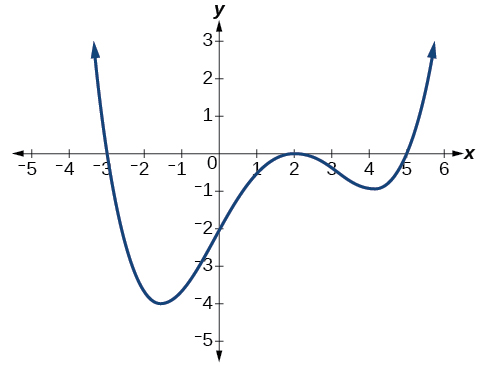
\includegraphics[scale=1]{Chapter 5/5.3-figure7.jpeg}



\end{document}


